\chapter{Autoencoders}

\begin{figure}[H]
    \centering
    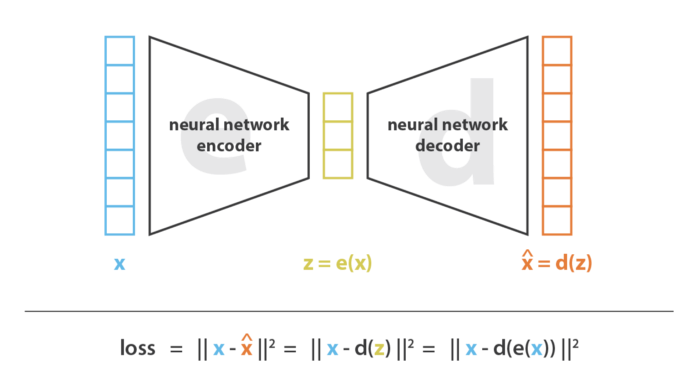
\includegraphics[width=10cm]{images/ae.png}
    \caption{Autoencoder}
    \label{fig:autoencoder}
\end{figure}

\section{Linear Autoencoders VS PCA}


\section{欠完备自编码器}
编码维度小于输入维度。学习欠完备的表示将强制自编码器捕捉训练数据中\textbf{最显著的特征},可用于\textbf{降维}。

\section{Undercomplete Autoencoders}
如果隐藏层的编码的维度允许与输入相等,或隐藏编码维数大于输入的过完备的情况下,会学习将输入复制到输出,而学不到任何有关数据分布的的有用信息。
正则自编码器使用的损失函数可以鼓励模型学习其他特性(除了将输入复制到输出),而不必限制使用浅层的编码器和解码器以及小的编码维度来限制模型的容量。这些
特性包括稀疏表示、表示的小导数以及对噪声或输入缺失的鲁棒性,即使模型容量大到足以学习一个无意义的恒等函数,非线性
且过完备的正则自编码器仍然能够从数据中学到一些关于数据分布的有用信息。

\subsection{Sparse Autoencoders}
\begin{equation}
    L(\vx, D(E(\vx))) + \Omega (h)
\end{equation}


\subsection{DAE - Denoising Autoencoders}
\begin{equation}
    L(\vx, D(E(\tilde{\vx})))
\end{equation}
$\hat{\vx}$ is a copy of $\vx$ that has been corrupted by some form of noise.


\subsection{CAE - Contractive Autoencoders}
\begin{equation}
    \begin{split}
        L(\vx, D(E(\vx))) + \Omega(\vh, \vx) \\
        \Omega(\vh, \vx) = \lambda \sum_i \| \nabla_x h_i \|^2
    \end{split}
\end{equation}

